\documentclass[notitlepage, 12pt]{article}

\usepackage{amssymb}           % dodatni simboli
\usepackage{amsmath}           % eqref, npr.
\usepackage[pdftex]{graphicx}
\usepackage{amsthm}
\usepackage{tikz}
\usepackage[dvipsnames]{xcolor}
\usepackage{svg}
\usepackage{fancyhdr}
\usepackage[normalem]{ulem}
\usepackage[hidelinks]{hyperref}

\usetikzlibrary{decorations.pathreplacing}
\usetikzlibrary{decorations.pathmorphing}


\usepackage{geometry}
\geometry{
  a4paper,
  total={160mm,257mm}, % total width and height of the text
  left=25mm, % left margin
  right=25mm, % right margin
}

\pagestyle{fancy}
\fancyhead{}
\fancyfoot[R]{Predavanje 1}
% remove the header line
\renewcommand{\headrulewidth}{0pt}


\graphicspath{ {./img/} }

\title{Teorija grafov - Zapiski predavanj}
\author{Jakob Drusany}

\newtheorem*{definition}{Definition}
\newtheorem*{theorem}{Theorem}
\newtheorem*{lemma}{Lemma}
\newtheorem*{example}{Example}
\newtheorem*{corollary}{Corollary}

\begin{document}
\maketitle
\vspace{1cm}
\tableofcontents
\thispagestyle{empty}
\newpage
\pagenumbering{arabic} 
\section{Introduction}
A graph is defined as $G = (V, E)$. $n = |V|$ is the number of vertices, $m = |E|$ is the number of edges.
We also denote them as $V(G), n(G)$, $E(G), m(G)$. $\delta(G)$ is the minimum degree of a vertex in $G$, $\Delta(G)$ is the maximum degree.
$G[C]$ represents the induced subgraph of $G$ on the vertex set $C$.
\section{Independence, matching, covers}
\begin{definition}
  The set of vertices $S \subseteq V$ is an \textbf{independent set} if $G(S)$ contains no edges.
  (No two vertices in the independent set are adjacent)
\end{definition}
The independence number $\alpha(G)$ is the size of the maximum independent set.
\begin{definition}
The set of vertices $T \subseteq V$ is a \textbf{vertex cover} if $\forall e \in E$ $T \cap e \neq \emptyset$.
(All edges have at least one endpoint in the vertex cover)
\end{definition}
The vertex cover number $\beta(G)$ is the size of the minimum vertex cover.
\begin{definition}
  A \textbf{matching} is a set of edges $M \subseteq E$ such that $\forall e, f \in M$ $e\neq f$ $e\cap f\neq \emptyset$.
  (No two edges share a vertex)
\end{definition}
The matching number $\alpha'(G)$ is the size of the maximum matching.
\begin{definition}
  An \textbf{edge cover} is a set of edges $C \subseteq E$ such that $\forall v \in V$ $\exists e \in C$ $v \in e$.
  (All vertices are covered by at least one edge from $C$)
\end{definition}
The edge cover number $\beta'(G)$ is the size of the minimum edge cover.
Some graphs have no edge covers, for example graphs with isolated vertices.

\begin{example}
    \begin{figure}[h]
      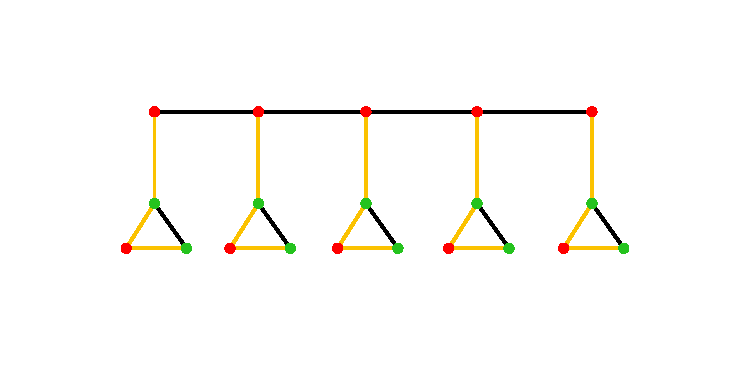
\includegraphics[width=0.8\textwidth]{first_example.pdf}
      \centering
      \caption{$G$ from example}
    \end{figure}

    % text colored red
    \textcolor{BrickRed}{$\alpha(G) = 8$}\\
    \textcolor{blue}{$h(G) = 20$}\\
    \textcolor{OliveGreen}{$\beta(G) = 12$} $\rightarrow$ complement of vertex set\\
    \textcolor{Dandelion}{$\alpha'(G) = 10$} maximum for $\alpha'$ is $\frac{h(G)}{2}$\\
    \textcolor{purple}{$\beta'(G) = 10$}
\end{example}
\newpage
\Large{Observations} \normalsize
\begin{itemize}
  \item $\alpha(G) + \beta(G) = |V|$ (the size of the maximum independent set plus the size of the minimum vertex cover is equal to the number of vertices)
  \begin{proof}
    For every independent set $S$, the complement $\overline{S}$ is a vertex cover and vice versa.
  \end{proof}
  $\alpha'(G) \leq \beta(G)$ (the size of the maximum matching is less than or equal to the size of the minimum vertex cover)
  \begin{figure}[h]
    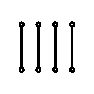
\includegraphics[width=0.2\textwidth]{matching-number-smaller-than-vertex-cover.pdf}
    \centering
  \end{figure}
  \begin{proof}
    Every edge in a maximum matching must be covered by different vertices in the vertex cover.
  \end{proof}
  \item \MakeLinkTarget{}\label{alpha-leq-betaline} $\alpha(G) \leq \beta'(G)$ (the size of the maximum independent set is less than or equal to the size of the minimum edge cover)
  \begin{proof}
    Every vertex in a maximum independent set must be covered by different edges in the edge cover.
  \end{proof}
  \item if $G$ has no isolated vertices: $\alpha'(G) \leq \frac{n}{2} \leq \beta(G)$
  \begin{figure}[h]
    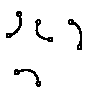
\includegraphics[width=0.2\textwidth]{matching-number-smaller-than-vertex-cover-2.pdf}
    \centering
  \end{figure}
\end{itemize}
\newpage
\section{Matchings}
\begin{theorem}[Galloi's theorem]\MakeLinkTarget{}\label{gallois-theorem}
  If $G$ has no isolated vertices, then $\alpha'(G) + \beta'(G) = n(G)$.
\end{theorem}
\begin{proof}
\begin{itemize}
    \item[(1)] $\beta'(G) + \alpha'(G) \leq |V(G)|$ \\ \newline
    \begin{figure}[h]
      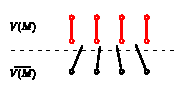
\includegraphics[width=0.4\textwidth]{gallois-theorem-1.pdf}
      \centering
    \end{figure}
    Take a maximum matching $M$; $M = \alpha'(G)$. For every vertex not covered
    in $M$ ($\overline{V(M)}$), we can take an incident edge and add them to $M$.
    We get a set of edges $R$, which covers every vertex in $G$.
    \begin{align*}
      |R| &= |M| + |\overline{V(M)}| = |M| + (|V(G)| - 2|M|)\\
      &= |V(G)| - |M|\\
      \beta'(&G) \leq |R| = |V(G)| - \alpha'(G)\\
      \beta'(&G) + \alpha'(G) \leq |V(G)|\\
    \end{align*}
  \item[(2)] $\beta'(G) + \alpha'(G) \geq |V(G)|$ \\ \newline
  \begin{lemma}
    Let $C$ be a minimum edge cover. For every edge in $C$, at least one of its
    endpoints is covered only once by $C$.
  \end{lemma}
  \begin{proof}
    Suppose $uv \in G$ and $u$ and $v$ are covered by other edges in $C$.
    $C' = C\ \{uv\}$ is also an edge cover and $|C'| < |C|$ which is a contradiction.
  \end{proof}
  Because of this, we can see that $G[C]$ is a star forest (for all minimal edge covers).
  \begin{figure}[h]
    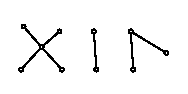
\includegraphics[width=0.4\textwidth]{gallois-part-2-star.pdf}
    \centering
  \end{figure}
  $G[C]$ consists of $k$ components: $|C| = |V(G)| - k$. A matching is obtained
  by chosing one edge from every star component of $G[C]$, the resulting matching
  has $k$ edges ($|M|$ = $k$)
  \begin{equation*}
    \alpha'(G) \geq |M| = k \geq |V(G)| -|C| = |V(G)| - \beta'(G)\\
  \end{equation*}
  \begin{equation*}
    \alpha'(G) + \beta'(G) \geq |V(G)|
  \end{equation*}
\end{itemize}
\end{proof}
\newpage
\section{Matchings}
Structure of the maximum matching $M$. For each $uv \in M$ one of these holds:
\begin{itemize}
\item[(1)] 
\begin{minipage}{.5\textwidth}
  \[
    N(u) \cap \overline{V(M)} = \emptyset
  \]
  \[
    N(v) \cap \overline{V(M)} = \emptyset
  \]
\end{minipage}% This must go next to `\end{minipage}`
\begin{minipage}{.5\textwidth}
  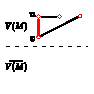
\includegraphics[width=0.45\textwidth]{max-matching-structure-1.pdf}
  \centering
\end{minipage}

\item[(2)] 
\begin{minipage}{.5\textwidth}
  \[
    N(u) \cap \overline{V(M)} \neq \emptyset
  \]
  \[
    N(v) \cap \overline{V(M)} \neq \emptyset
  \]
\end{minipage}% This must go next to `\end{minipage}`
\begin{minipage}{.5\textwidth}
  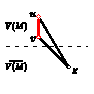
\includegraphics[width=0.45\textwidth]{max-matching-structure-2.pdf}
  \centering
\end{minipage}

\item[(3)]
\begin{minipage}{.20\textwidth}
  \[
    N(u) \cap \overline{V(M)} \neq \emptyset
  \]
  \[
    N(v) \cap \overline{V(M)} = \emptyset
  \]
\end{minipage}% This must go next to `\end{minipage}`
\begin{minipage}{.05\textwidth}
  or
  \centering
\end{minipage}% This must go next to `\end{minipage}`
\begin{minipage}{.20\textwidth}
  \[
    N(u) \cap \overline{V(M)} = \emptyset
  \]
  \[
    N(v) \cap \overline{V(M)} \neq \emptyset
  \]
\end{minipage}% This must go next to `\end{minipage}`
\begin{minipage}{.6\textwidth}
  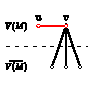
\includegraphics[width=0.45\textwidth]{max-matching-structure-3.pdf}
  \centering
\end{minipage}
\end{itemize}
\begin{definition}
Let $M$ be a matching. A path $v_1u_1v_2u_2\dots v_k u_k (v_{k+1})$ is an \textbf{m-altering path} if the edges along
the path alternate between $M$ and $\overline{M} = E \ M$
\end{definition}
\begin{figure}[h]
  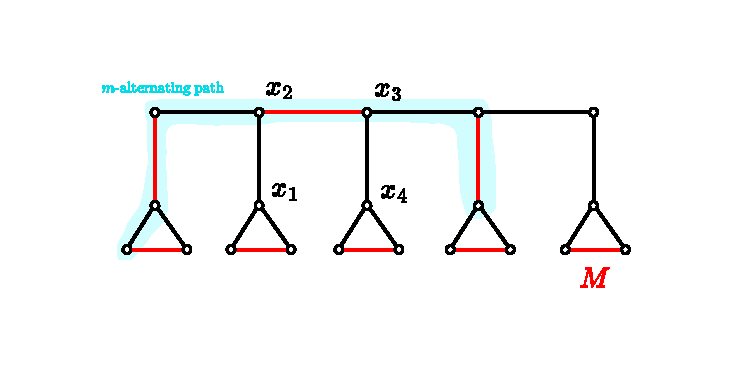
\includegraphics[width=0.8\textwidth]{m-alternating-example.pdf}
  \centering
\end{figure}
\begin{definition}
  An $m$-alternating path is $m$-augmenting if both ends of the path are uncovered by $M$
\end{definition}
For example $x_1x_2x_3x_4$ in the above figure.
This is important because $M'=M \setminus \{x_2x_3\}\cup \{x_1x_2\}$
is a larger matching.
\newpage
\fancyfoot[R]{Predavanje 2}
\begin{theorem}\MakeLinkTarget{}\label{thm:theorem-augmenting-to-maximum}
  Let $G$ be a graph and $M$ a matching in $G$. If there exists an $M$-augmenting path
  then $M$ is not a maximum matching.
\end{theorem}
\begin{center}
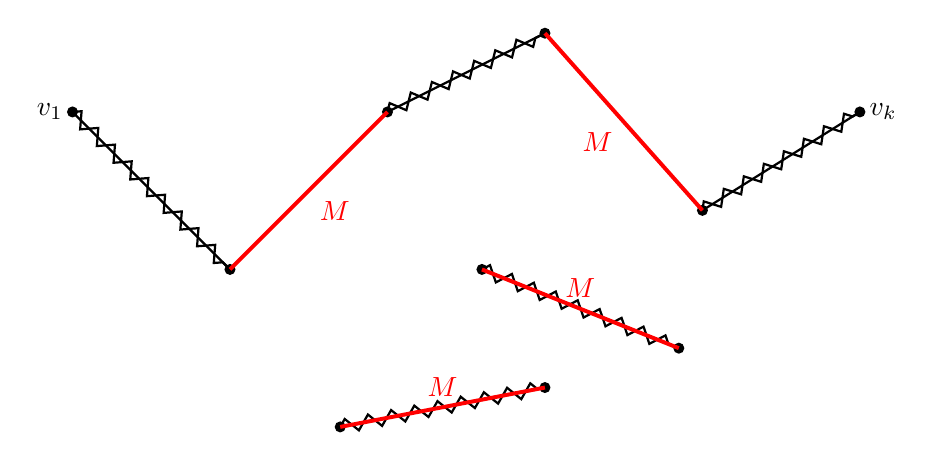
\begin{tikzpicture}
  % 6 vertices 
  \coordinate(p1) at (0,0);
  \coordinate(p2) at (2,-2);
  \coordinate(p3) at (4,0);
  \coordinate(p4) at (6,1);
  \coordinate(p5) at (8,-1.25);
  \coordinate(p6) at (10,0);

  \coordinate(a1) at (3.4,-4);
  \coordinate(a2) at (6,-3.5);

  \coordinate(b1) at (5.2,-2);
  \coordinate(b2) at (7.7,-3);

  % Draw the pertices
  \fill (p1) circle (2pt) node[left] {$v_1$};
  \fill (p2) circle (2pt) node[below] {};
  \fill (p3) circle (2pt) node[below] {};
  \fill (p4) circle (2pt) node[below] {};
  \fill (p5) circle (2pt) node[below] {};
  \fill (p6) circle (2pt) node[right] {$v_k$};

  \fill (a1) circle (2pt) node[below] {};
  \fill (a2) circle (2pt) node[below] {};

  \fill (b1) circle (2pt) node[below] {};
  \fill (b2) circle (2pt) node[below] {};

  % highlight the p1-p2 edges in a different way
  \draw[thick, black, decorate, decoration={zigzag, segment length=3mm}] (p1) -- (p2);
  \draw[thick, black, decorate, decoration={zigzag, segment length=3mm}] (p3) -- (p4);
  \draw[thick, black, decorate, decoration={zigzag, segment length=3mm}] (p5) -- (p6);

  \draw[thick, black, decorate, decoration={zigzag, segment length=3mm}] (a1) -- (a2);
  \draw[thick, black, decorate, decoration={zigzag, segment length=3mm}] (b1) -- (b2);

  % Draw the edges
  \draw[thick] (p1) -- (p2) -- (p3) -- (p4) -- (p5) -- (p6);

  \draw[line width=0.5mm, red] (p2) -- (p3) node[midway, below right] {$M$};
  \draw[line width=0.5mm, red] (p4) -- (p5) node[midway, below left] {$M$};

  \draw[line width=0.5mm, red] (a1) -- (a2) node[midway, above] {$M$};
  \draw[line width=0.5mm, red] (b1) -- (b2) node[midway, above] {$M$};
\end{tikzpicture}
\end{center}
\begin{proof}
  Let $P$ be an $M$-augmenting path. $P = v_1v_2\dots v_k$, because it is an augmenting path
  $v_1v_2 \notin M$ $v_{k-1}v_k \notin M$ $\Rightarrow |E(P) \cap \overline{M}| = |E(P) \cap M|+1$
  \noindent
  Let $M' = M \Delta E(P)$, $M'$ is a matching in $G$ (Marked as zigzag lines in the graph).

  \noindent
  \dashuline{$M'$ is a matching}
  \begin{itemize}
    \item For vertices outside $P$ the edges are the same in $M$ and $M'$.
    \item $v_1, v_k$ were uncovered by $M$ so they are now covered by $M'$.
    \item For internal vertices: $v_i$ is covered once in $M$. This edge is missing
    in $M'$, therefore $v_i$ is covered by another edge in $M'$.
  \end{itemize}
$\Rightarrow M'$ is a matching, $|M'| = |M| + 1$, so $M$ is not a maximum matching.
\end{proof}

König-Egerváry graphs:
\begin{center}

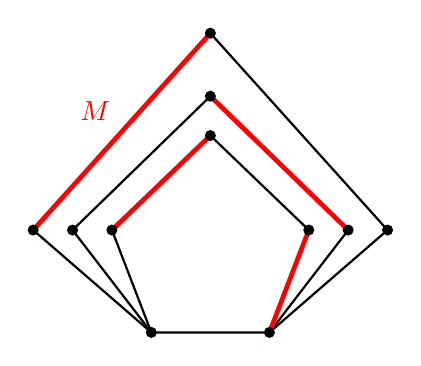
\begin{tikzpicture}
  \coordinate (p1) at (0,0);
  \coordinate (p2) at (1.5,0);
  % first cycle
  \coordinate (p3) at (-0.5,1.3);
  \coordinate (p4) at (2,1.3);
  \coordinate (p5) at (0.75,2.5);
  % second cycle
  \coordinate (p6) at (-1,1.3);
  \coordinate (p7) at (2.5,1.3);
  \coordinate (p8) at (0.75,3);
  % third cycle
  \coordinate (p9) at (-1.5,1.3);
  \coordinate (p10) at (3,1.3);
  \coordinate (p11) at (0.75,3.8);
  
  
  \draw[thick] (p1) -- (p2) -- (p4) -- (p5) -- (p3) -- (p1);
  \draw[thick] (p2) -- (p7) -- (p8) -- (p6) -- (p1);
  \draw[thick] (p2) -- (p10) -- (p11) -- (p9) -- (p1);

  % highlight the matching
  \draw[line width=0.6mm, red] (p3) -- (p5);
  \draw[line width=0.6mm, red] (p2) -- (p4);
  \draw[line width=0.6mm, red] (p7) -- (p8);
  \draw[line width=0.6mm, red] (p9) -- (p11) node[midway, above left] {$M$};
  
  \foreach \i in {1,...,11} {
    \fill (p\i) circle (2pt);
  }
  \end{tikzpicture}
\end{center}

König-Egerváry have $\alpha'(G) = \beta(G)$. In the example: $\alpha'(G) = 5 = \beta(G)$, $G$ is not bipartite.
\begin{theorem}[Königs theorem]\MakeLinkTarget{}\label{konigs-theorem}
  Let $G$ be a bipartite graph, then the following holds:
  \begin{itemize}
    \item[(a)] $\alpha'(G) = \beta(G)$
    \item[(b)] let $M$ be a matching in $G$ and a $M$-augmenting path does not exist, then
    $M$ is a maximum matching.
  \end{itemize}
\end{theorem}
\begin{proof}
Let $G$ be a bipartite graph on sets $A,B$. Suppose that $M$ is a matching such that
  an $M$-augmenting path in $G$ does not exist (such an $M$ exists).
  \begin{center}
    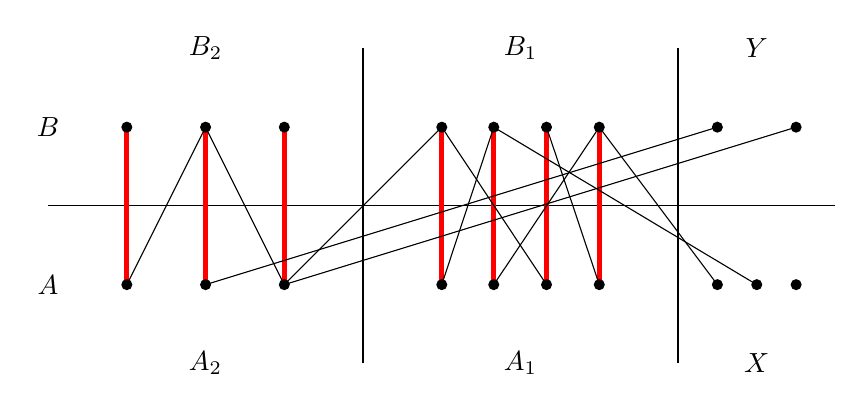
\begin{tikzpicture}
      % split into A,B and 3 groups (A,B,xy)
      \draw (0,0) -- (10,0);
      \draw (4,-2) -- (4,2);
      \draw (8,-2) -- (8,2);

      %write A,B
      \node at (0,-1) {$A$};
      \node at (0,1) {$B$};

      %write B2, A2
      \node at (2,2) {$B_2$};
      \node at (2,-2) {$A_2$};

      %write B1, A1
      \node at (6,2) {$B_1$};
      \node at (6,-2) {$A_1$};

      %write x,y
      \node at (9,2) {$Y$};
      \node at (9,-2) {$X$};

      % draw 3 nodes horizontally in B2 and 3 in A2
      \coordinate (B21) at (1,1);
      \coordinate (B22) at (2,1);
      \coordinate (B23) at (3,1);
      \coordinate (A21) at (1,-1);
      \coordinate (A22) at (2,-1);
      \coordinate (A23) at (3,-1);

      % draw 3 node horizontally in B1 and 3 in A1
      \coordinate (B11) at (5,1);
      \coordinate (B12) at (5.66,1);
      \coordinate (B13) at (6.33,1);
      \coordinate (B14) at (7,1);
      \coordinate (A11) at (5,-1);
      \coordinate (A12) at (5.66,-1);
      \coordinate (A13) at (6.33,-1);
      \coordinate (A14) at (7,-1);
      
      % draw 2 nodes in y and 3 nodes in x
      \coordinate (y1) at (8.5,1);
      \coordinate (y2) at (9.5,1);
      \coordinate (x1) at (8.5,-1);
      \coordinate (x2) at (9,-1);
      \coordinate (x3) at (9.5,-1);

      \fill (y1) circle (2pt);
      \fill (y2) circle (2pt);
      \fill (x1) circle (2pt);
      \fill (x2) circle (2pt);
      \fill (x3) circle (2pt);

      % connections in matching
      \draw[line width=0.6mm, red] (B21) -- (A21);
      \draw[line width=0.6mm, red] (B22) -- (A22);
      \draw[line width=0.6mm, red] (B23) -- (A23);
      \draw[line width=0.6mm, red] (B11) -- (A11);
      \draw[line width=0.6mm, red] (B12) -- (A12);
      \draw[line width=0.6mm, red] (B13) -- (A13);
      \draw[line width=0.6mm, red] (B14) -- (A14);

      % connections between nodes
      \draw (B22) -- (A21);
      \draw (B22) -- (A23);

      \draw (A22) -- (y1);
      \draw (A23) -- (y2);

      \draw (B11) -- (A13);
      \draw (B12) -- (A11);
      \draw (B13) -- (A14);
      \draw (B14) -- (A12);
      \draw (B12) -- (x2);
      \draw (B14) -- (x1);
      \draw (A23) -- (B11);

      \fill (B21) circle (2pt);
      \fill (B22) circle (2pt);
      \fill (B23) circle (2pt);
      \fill (A21) circle (2pt);
      \fill (A22) circle (2pt);
      \fill (A23) circle (2pt);
      \fill (B11) circle (2pt);
      \fill (B12) circle (2pt);
      \fill (B13) circle (2pt);
      \fill (B14) circle (2pt);
      \fill (A11) circle (2pt);
      \fill (A12) circle (2pt);
      \fill (A13) circle (2pt);
      \fill (A14) circle (2pt);
    \end{tikzpicture}
  \end{center}
  \begin{itemize}
    \item $M$ is marked in red
    \item $x,y$ are the sets of uncovered vertices in $A,B$ ($X = A \setminus V(M)$, $Y = B \setminus V(M)$).
    \item $B_1$ is the set of vertices in $B$ that are reachable from $X$ with an $M$-alternating path.
    \item $A_1$ is the set of vertices in $A$ that are reachable from $X$ with an $M$-alternating path.
    \item $B_2 = B \setminus (B_1 \cup Y)$
    \item $A_2 = A \setminus (A_1 \cup X)$
  \end{itemize}
  $A \rightarrow B$ edges are in $\overline{M}$ \\
  $B \rightarrow A$ edges are in $M$ \\

  \noindent $A_1 = \{ a\in A\ |\ \exists b \in B_1: ab \in M \}, \quad A_2 = \{ a\in A\ |\ \exists b \in B_2: ab \in M \}$\\

  $|A_1| = |B_1|$;\quad $|A_2| = |B_2|$; \quad$|A_1| + |A_2| = |M|$\\

  We can prove that the following statements hold:
  \begin{itemize}
    \item There are no edges between $X$ and $Y$ \\
    Lets propose $x \in X, y \in Y, xy \in E$. This is an $M$-alternating path of length 1.
    It is also an $M$-augmenting path, because its endpoints are not covered by $M$. This
    is a contradiction, because we assumed that there are no $M$-augmenting paths.
    \item There are no edges between $X$ and $B_2$ \\
    An edge $x\in X,b\in B2, xb\in E$ is an $M$-alternating path from $X$ to $B_2$ which 
    contradicts the definition of $B_1$ and $B_2$.
    \newpage
    \item There are no edges between $A_1$ and $Y$ \\
    Suppose that $a\in A_1, y\in Y, ay\in E$.

    \begin{center}
    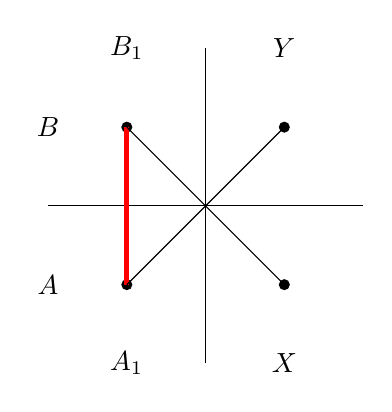
\begin{tikzpicture}
      \draw (0,0) -- (4,0);
      \draw (2,-2) -- (2,2);

      %write A,B
      \node at (0,-1) {$A$};
      \node at (0,1) {$B$};

      %write B1, A1
      \node at (1,2) {$B_1$};
      \node at (1,-2) {$A_1$};

      %write x,y
      \node at (3,2) {$Y$};
      \node at (3,-2) {$X$};

      % draw 3 node horizontally in B1 and 3 in A1
      \coordinate (B11) at (1,1);
      \coordinate (A11) at (1,-1);
      \coordinate (Y1) at (3,1);
      \coordinate (X1) at (3,-1);

      \fill (B11) circle (2pt);
      \fill (A11) circle (2pt);
      \fill (Y1) circle (2pt);
      \fill (X1) circle (2pt);

      % connections in matching
      \draw[line width=0.6mm, red] (B11) -- (A11);

      % connections between nodes
      \draw (B11) -- (X1);
      \draw (A11) -- (Y1);
    \end{tikzpicture}
  \end{center}

    There exists an $M$-alternating path from $X$ to $B_1$:
    \[v_1v_2\dots v_k,\ v_1 \in X,\ v_k \in B_1\]
    We can now add an edge from $v_k$ to $a$ from the matching $M$ and $ay$ not from $M$.
    The path
    \[v_1v_2\dots v_kay\]
    is an $M$-alternating path and because $v_1$ and $y$ are not covered by $M$ it is also an $M$-augmenting path.
    \item There are no edges between $A_1$ and $B_2$ \\
    If we begin an $M$-alternating path in $X$ and end in $A_1$ we get a path:
    \[xv_2\dots v_{k-1}a,\ x \in X,\ a \in A_1\]
    Now we can add the edge $ab, b\in B_1, ab \notin M$. We know that $v_{k-1}a \in M$ so
    $x_1v_2\dots v_{k-1}ab$ is an $M$-alternating path. $B_1$ is therefore reachable from $X$ with
    an $M$-alternating path. This a contradiction with the definition
    of $B_1$ and $B_2$.
  \end{itemize}

  \noindent\dashuline{$T=B_1 \cup A_2$ is a vertex cover}\\
  We only need to prove that all edges from $A = X\cup A_1\cup A_2$ are covered by the vertex cover because the graph
  is a bipartite graph.
  \begin{itemize}
    \item all edges from $X$ are covered by a vertex in $B_1$
    \item all edges from $A_1$ are covered by a vertex in $B_1$
    \item all edges from $A_2$ are covered by a vertex in $A_2$
  \end{itemize}

  Now we can finish the proof:
  \[|T| = |B_1|+|A_2| = |A_1|+|A_2|=|M|\]
  \[\beta(G) \leq |T| = |M| \leq \underbrace{\alpha'(G) \leq \beta(G)}_{\text{\hyperref[alpha-leq-betaline]{proven}}}\]
  From this we can conclude:
  \begin{itemize}
    \item[(a)] $\alpha'(G) = \beta(G)$
    \item[(b)] $|M| = \alpha'(G)$ therefore $M$ is a maximum matching.
  \end{itemize}
\end{proof}
\begin{corollary}
  If $G$ is a bipartite graph then $\alpha(G) = \beta'(G)$.
\end{corollary}
\begin{proof}
  \[\alpha(G) = n(G) - \beta(G) \stackrel{ \stackrel{\text{Königs}}{\downarrow} }{=} n(G) - \alpha'(G) \stackrel{ \stackrel{\text{\hyperref[gallois-theorem]{Gallois}}}{\downarrow} }{=} \beta'(G)\]
\end{proof}
\begin{definition}[HC]
  $G$ is a bipartite on the sets $A,B$. \textbf{Halls condition (HC)} holds for $A$ if 
  \[\forall S \subseteq A:\quad |S| \leq |N(G)|\]
  where $N(S) = \cup_{x\in S} N(x)$ is the set of neighbors of $S$.
\end{definition}
\begin{theorem}[Halls theorem]
  $G$ bipartite on $A,B$. There exists a matching that covers $A \iff$ HC holds for $A$.
\end{theorem}
\begin{proof}\hfill

  \begin{itemize}
    \item[($\Rightarrow$)] Let $M$ be the matching that covers $A$. $\forall S \subseteq A$ we can take
    the pairs matched by $M$:
    \[ B_S = \{ v\in B\ |\ \exists u\in S: uv\in M\} \]
    We know that $|S| = |B_S|$ and $B_S \subseteq N(S) \Rightarrow |S| = |B_S| \leq |N(S)|$. Therefore HC holds for $A$.
    \item[($\Leftarrow$)] We have to prove that there does not exist a matching $M$ that covers $A \Rightarrow$ HC does not hold for $A$ \\ Take the maximum matching in $G$. Lets draw the same picture for $G$ as in the proof of \hyperref[konigs-theorem]{Königs theorem}.
    \begin{center}
      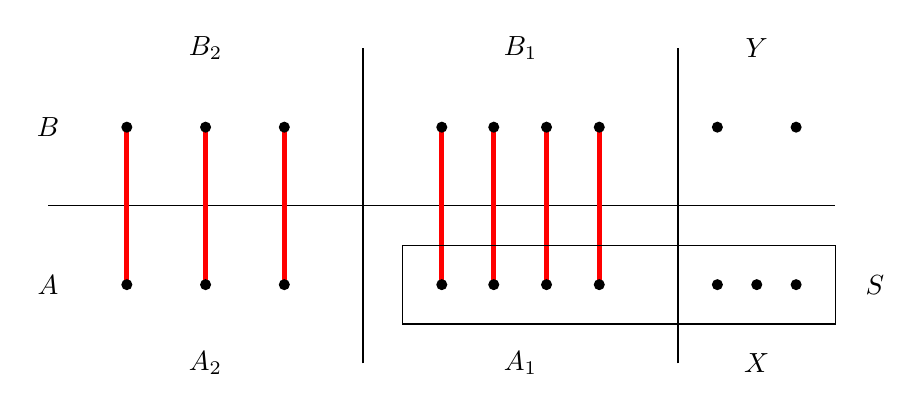
\begin{tikzpicture}
        % split into A,B and 3 groups (A,B,xy)
        \draw (0,0) -- (10,0);
        \draw (4,-2) -- (4,2);
        \draw (8,-2) -- (8,2);
  
        %write A,B
        \node at (0,-1) {$A$};
        \node at (0,1) {$B$};
  
        %write B2, A2
        \node at (2,2) {$B_2$};
        \node at (2,-2) {$A_2$};
  
        %write B1, A1
        \node at (6,2) {$B_1$};
        \node at (6,-2) {$A_1$};
  
        %write x,y
        \node at (9,2) {$Y$};
        \node at (9,-2) {$X$};
  
        % draw 3 nodes horizontally in B2 and 3 in A2
        \coordinate (B21) at (1,1);
        \coordinate (B22) at (2,1);
        \coordinate (B23) at (3,1);
        \coordinate (A21) at (1,-1);
        \coordinate (A22) at (2,-1);
        \coordinate (A23) at (3,-1);
  
        
        % draw 3 node horizontally in B1 and 3 in A1
        \coordinate (B11) at (5,1);
        \coordinate (B12) at (5.66,1);
        \coordinate (B13) at (6.33,1);
        \coordinate (B14) at (7,1);
        \coordinate (A11) at (5,-1);
        \coordinate (A12) at (5.66,-1);
        \coordinate (A13) at (6.33,-1);
        \coordinate (A14) at (7,-1);
        
        % draw 2 nodes in y and 3 nodes in x
        \coordinate (y1) at (8.5,1);
        \coordinate (y2) at (9.5,1);
        \coordinate (x1) at (8.5,-1);
        \coordinate (x2) at (9,-1);
        \coordinate (x3) at (9.5,-1);
  
        \fill (y1) circle (2pt);
        \fill (y2) circle (2pt);
        \fill (x1) circle (2pt);
        \fill (x2) circle (2pt);
        \fill (x3) circle (2pt);
  
        % connections in matching
        \draw[line width=0.6mm, red] (B21) -- (A21);
        \draw[line width=0.6mm, red] (B22) -- (A22);
        \draw[line width=0.6mm, red] (B23) -- (A23);
        \draw[line width=0.6mm, red] (B11) -- (A11);
        \draw[line width=0.6mm, red] (B12) -- (A12);
        \draw[line width=0.6mm, red] (B13) -- (A13);
        \draw[line width=0.6mm, red] (B14) -- (A14);

        \fill (B21) circle (2pt);
        \fill (B22) circle (2pt);
        \fill (B23) circle (2pt);
        \fill (A21) circle (2pt);
        \fill (A22) circle (2pt);
        \fill (A23) circle (2pt);
        \fill (B11) circle (2pt);
        \fill (B12) circle (2pt);
        \fill (B13) circle (2pt);
        \fill (B14) circle (2pt);
        \fill (A11) circle (2pt);
        \fill (A12) circle (2pt);
        \fill (A13) circle (2pt);
        \fill (A14) circle (2pt);

        % draw a rounded square around the nodes of A1 and X
        \draw (4.5,-0.5) rectangle (10,-1.5);

        % write S on the right edge of the square
        \node at (10.5,-1) {$S$};

      \end{tikzpicture}
    \end{center}
    The maximum matching does not cover $A \Rightarrow X \neq \emptyset$. Consider $S = A_1 \cup X$.
    We have seen that all neighbors of $S$ are in $B_1$ (in \hyperref[konigs-theorem]{Königs}) so 
    $N(S) = B_1$, $|S| = |A_1| + |X|$ and $|N(S)| = |B_1| = |A_1|$ so $|S| > |N(S)|$ which
    means that HC does not hold for $A$.
  \end{itemize}
\end{proof}
\newpage
\fancyfoot[R]{Predavanje 3}
\begin{theorem}
Let $M$ be a matching in $G$. There exists an $M$-augmenting path
$\iff$ $M$ is not a maximum matching.
\end{theorem}
\begin{proof}
\begin{itemize}
  \item[($\Rightarrow$)] this was proven in \hyperref[thm:theorem-augmenting-to-maximum]{the previous lecture}
  \item[($\Leftarrow$)] $M$ is a matching, not maximum. Then there exists a  $M'$ matching 
  such that $|M'| > |M|$. Consider $M \Delta M'$ (symmetric difference).
  Let $G' = G[M \Delta M']$. In $G'$, the maximum degree $\Delta(G') \leq 2$. $G'$ contains
  only paths and cycles. If The component is a cycle:

  \begin{center}
    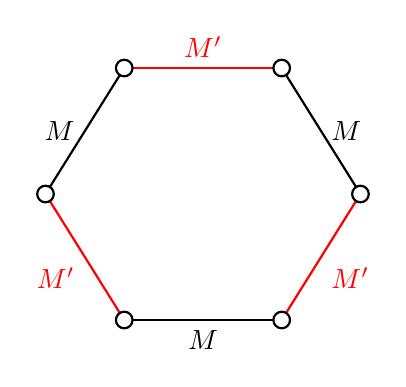
\begin{tikzpicture}
      % Coordinates for the hexagon vertices in the desired positions
      \coordinate (A) at (-1,1.6);  % Top left
      \coordinate (B) at (1,1.6);   % Top right
      \coordinate (C) at (-2,0);  % Left
      \coordinate (D) at (2,0);   % Right
      \coordinate (E) at (-1,-1.6); % Bottom left
      \coordinate (F) at (1,-1.6);  % Bottom right
  
      % Draw hexagon with alternating line colors
      \draw[thick, red] (A) -- (B) node[midway, above] {$M'$};   % Top red line
      \draw[thick, black] (E) -- (F) node[midway, below] {$M$};    % Bottom red line
      \draw[thick, black] (B) -- (D) node[midway, right] {$M$};  % Right black line
      \draw[thick, red] (D) -- (F) node[midway, below right] {$M'$}; % Bottom-right black line
      \draw[thick, black] (A) -- (C) node[midway, left] {$M$};   % Left black line
      \draw[thick, red] (C) -- (E) node[midway, below left] {$M'$};  % Bottom-left black line
      
      % Draw circles at vertices
      \foreach \point in {A, B, C, D, E, F} {
          \fill[white] (\point) circle (3pt);
          \draw[thick] (\point) circle (3pt);
      }
  
  \end{tikzpicture}
  \end{center}

  $M$ and $M'$ edges alternate in the cycle, therefore there are the same number of edges from $M$ and $M'$ in the cycle.\\
  If The component is a path:
  \begin{itemize}
    \item path of even length, then $M$,$M'$-edges alternate, therefore there are the same number of edges from $M$ and $M'$ in the path.
    \item path of odd length, then there is one more edge from $M'$ than from $M$ or vice versa.
  \end{itemize}
  \[|M'| > |M| \Rightarrow |M' \setminus M| > |M \setminus M'|\]
  $\Rightarrow$ there exists a component $G_1'$ in $G'$ such that there are more
  edges from $M'$ than from $M$. This component is a path of odd length that starts and
  ends with an edge from $M'$.
\begin{center}
  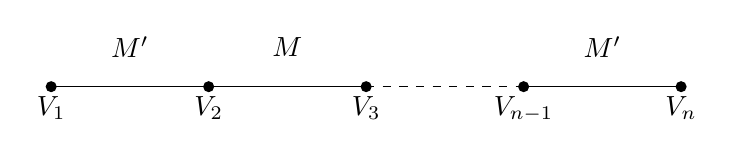
\begin{tikzpicture}
    % Define coordinates
    \coordinate (V1) at (0,0);
    \coordinate (V2) at (2,0);
    \coordinate (V3) at (4,0);
    \coordinate (Vn1) at (6,0);
    \coordinate (Vn) at (8,0);

    % Draw points
    \fill (V1) circle (2pt) node[below] {$V_1$};
    \fill (V2) circle (2pt) node[below] {$V_2$};
    \fill (V3) circle (2pt) node[below] {$V_3$};
    \fill (Vn1) circle (2pt) node[below] {$V_{n-1}$};
    \fill (Vn) circle (2pt) node[below] {$V_n$};

    % Draw lines between points
    \draw (V1) -- (V2);
    \draw (V2) -- (V3);
    \draw[dashed] (V3) -- (Vn1);
    \draw (Vn1) -- (Vn);

    % Add labels above points
    \node at (1,0.5) {$M'$};
    \node at (3,0.5) {$M$};
    \node at (7,0.5) {$M'$};
  \end{tikzpicture}
  \end{center}

  The following holds:
  \begin{itemize}
    \item $G_1'$ is an $M$-alternating path
    \item $v_1$ is not covered by $M$.
    \item in $G'$ $deg(v_1)=1$ (because it is a path component), therefore no
    edge from $M \setminus M'$ is incident to $v_1$.
    \item $v_1$ is not incident to any edge from $M \cap M'$ since $v_1$ is
    already covered by an edge from $M'$.
  \end{itemize}
  In conclusion $v_1, v_k$ are not covered by $M$ so $G_1'$ is an alternating
  path with uncovered endpoints and is therefore an $M$-augmenting path.
\end{itemize}
\end{proof}
Algorithms for the above theorems:
\begin{itemize}
  \item "Blossom algorithms" - to find an $M$-augmenting path and improve the matching
  if possible. The best known algorithm is $O(n\sqrt{n})$.
  \item We can determine the matching number and the edge cover number in polynomial time.
\end{itemize}
\vspace{1cm}
\begin{definition}[Oddity]
  $o(G)$: number of odd components in $G$
\end{definition}
\begin{theorem}[Tuttes theorem]
  $G$ has a perfect matching $\iff$ $\forall S \subseteq V(G)$ $o(G-S) \leq |S|$
\end{theorem}
$o(G-S) \leq |S|$ is called the Tutte condition.
\begin{proof}
  \begin{itemize}
    \item[($\Rightarrow$)] $M$ is a perfect matching in $G$. For every $S \subseteq V(G)$.
    \begin{figure}[h!]
    \centering
    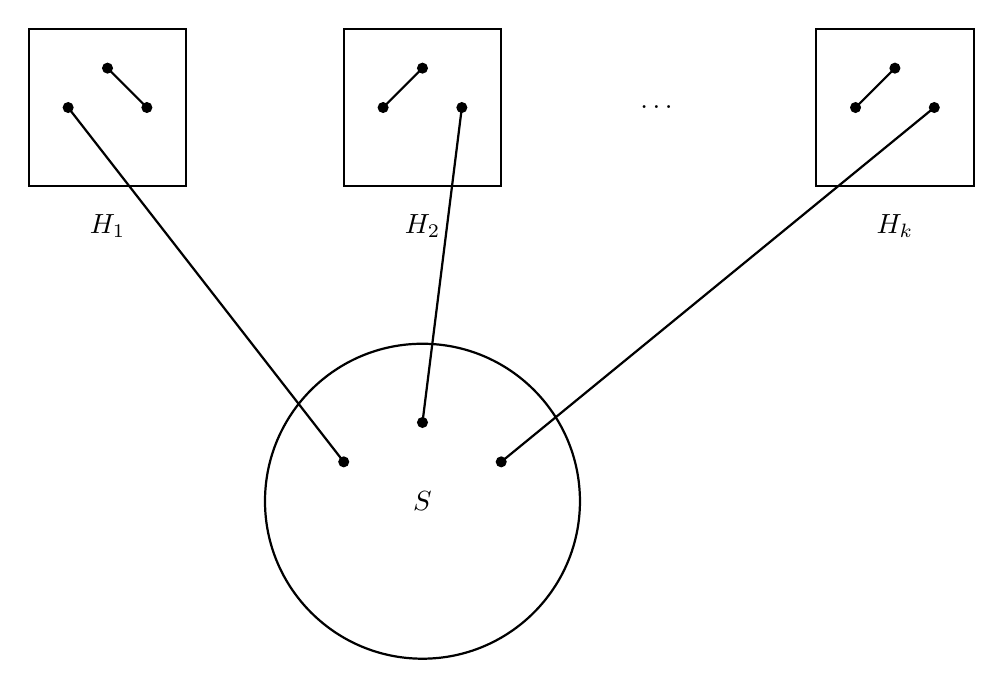
\begin{tikzpicture}
      % Draw the sets H1, H2, and Hk as rectangles
      \draw[thick] (-5,2) rectangle (-3,4) node[midway, below]{};
      \draw[thick] (-1,2) rectangle (1,4) node[midway, below]{};
      \draw[thick] (5,2) rectangle (7,4) node[midway, below]{};

      % write H1, H2, Hk under the rectangles
      \node at (-4,1.5) {$H_1$};
      \node at (0,1.5) {$H_2$};
      \node at (6,1.5) {$H_k$};
  
      % Draw the circle S
      \draw[thick] (0,-2) circle (2) node {$S$};
  
      % Connect lines from the left-over vertices of H1, H2, and Hk to the circle S
      \draw[thick] (-4.5,3) -- (-1,-1.5); % Leftover vertex from H1 to S
      \draw[thick] (0.5,3) -- (0,-1);   % Leftover vertex from H2 to S
      \draw[thick] (6.5,3) -- (1,-1.5);     % Leftover vertex from Hk to S

      % Draw vertices in S
      \fill (0,-1) circle (2pt); % S vertex
      \fill (-1,-1.5) circle (2pt); % S pair 1
      \fill (1,-1.5) circle (2pt);  % S pair 2
  
      % Draw vertices in H1, H2, Hk
      \fill (-4.5,3) circle (2pt); % H1 vertex leftover
      \fill (-4,3.5) circle (2pt); % H1 pair 1
      \fill (-3.5,3) circle (2pt); % H1 pair 2
      \draw[thick] (-4,3.5) -- (-3.5,3); % Connect pair in H1
  
      \fill (-0.5,3) circle (2pt); % H2 pair 1
      \fill (0,3.5) circle (2pt);  % H2 pair 2
      \fill (0.5,3) circle (2pt);  % H2 vertex leftover
      \draw[thick] (-0.5,3) -- (0,3.5); % Connect pair in H2
  
      \fill (5.5,3) circle (2pt); % Hk pair 1
      \fill (6,3.5) circle (2pt); % Hk pair 2
      \fill (6.5,3) circle (2pt);   % Hk vertex leftover
      \draw[thick] (5.5,3) -- (6,3.5); % Connect pair in Hk
  
      % Dots between H2 and Hk
      \node at (3,3) {$\dots$};
    \end{tikzpicture}
    \caption{Graph $G$ showing $S$ and $H_i$ which are odd components not in $S$}
    \end{figure}

    if $H_1$ is an odd component then there exists at least one $M$-edge between $V(H_i)$ and $S$.
    This holds for every odd component. Therefore there exists at least $o(G-S)$ $M$-edges
    between $S$ and $\overline{S}$. As $M$ is a matching these edges are incident do different
    vertices from $S$. Therefore $o(G-S) \leq |S|$ (Tuttes condition holds).
  
    \item[($\Leftarrow$)] If the Tuttes condition holds then there exists a perfect matching.
    Suppose that the lemma does not hold. Then there exists a counter example $F$ on $n$ vertices.
    \begin{itemize}
      \item[(1)] $F$ satisfies the Tuttes condition
      \item[(2)] There does not exist a perfect matching in $F$
    \end{itemize}
    We can add edges to $F$ while it remains a counter example, until we get a graph $G$. $G$ is then
    the largest counter example.
    \begin{lemma}
      $n(G)$ is even
    \end{lemma}
    \begin{proof}
      if we take $S = \emptyset$, then
      \[|S|=0 \geq o(G-s) = o(G) \geq 0 \quad \Rightarrow \quad o(G)=0\]
      Because the number of odd components is zero, $n$ is even.
    \end{proof}
    \begin{lemma}\MakeLinkTarget{}\label{proof-lemma:2}
      $\forall e \in E(\overline(G))$ $G'=G+e$ has a perfect matching
    \end{lemma}
    \begin{proof}
      \begin{itemize}
        \item $G+e$ is not a counter example (because of the maximality of $G$).
        \item $G+e$ satisfies TC:
        For every $S \subseteq V(G+e)$ $o(G+e-S) \leq |S|$.\\
        When adding an edge $e$ to $G$ we have 4 cases:
        \begin{itemize}
          \item[(a)] If the edge $e$ is inside $S$ or inside a component of $G-S$, then the number of
          odd components does not change.
          \item[(b)] If the edge $e$ is between two even components of $G-S$, then the number of odd components
          does not change.
          \item[(c)] If the edge $e$ is between odd-even components of $G-S$, then the number of odd components
          does not change.
          \item[(d)] If the edge $e$ is between two odd components of $G-S$, then the number of odd components
          decreases by two (the two odd components become an even component).
        \end{itemize}
        Therefore $G'$ satisfies the Tuttes condition:
        \[|S| \geq o(G-S) \geq o(G'- S)\]
      \end{itemize}
      $G'$ is not a counter example, therefore (2) does not hold and there exists a perfect matching in $G'$.
    \end{proof}
    To end the proof we need to show that $G$ has a perfect matching. Let $u$ be the set of
    universal vertices ($deg(v) = n-1$) in $G$. $G[u]$ is a complete graph (fully connected).
    We can construct a perfect matching for different cases:
    \begin{enumerate}
      \item If every $H_i$ induces a complete graph, then we can construct a matching $M$
      \begin{itemize}
        \item If $H_i$ is an even component then then we can cover every vertex with $M$-edges inside $H_i$.
        \item If $H_i$ is an odd component then we cover all but one vertex with $M$-edges inside $H_i$.
        \item The remaining $o(G-u)$ vertices fro the odd components can be covered with $M$-edges between $u$
        and the components using $o(G-u)$ different vertices from $u$. This can be done as all edges are present
        in $G$ between $u$ and $\overline{u}$ and $o(G-u) \leq |u|$.
        \item If some vertices from $u$ are uncovered then we define a matching on them. This is possible
        because $G[u]$ is a complete graph, $n(G)$ is even and $M$ covered an even number of vertices so far.
      \end{itemize}
      Therefore $G$ has a perfect matching.

      \item If there exists a non-complete component $H_i$, then we can find a pair of vertices $x,y$ such that
      $dist(x,y) = 2$.

      \begin{center}
        \begin{tikzpicture}

          % Left square
          \draw (0,0) rectangle (1,1);
          
          % Middle square with label w
          \draw (2,0) rectangle (3,1);
          \node at (2.5,0.6) {w};
          \fill (2.5,0.3) circle (2pt);
      
          % Right square
          \draw (7,0) rectangle (8,1);
      
          % Central square with points x, y, z
          \draw (4,0) rectangle (6,2);
          \node at (5,2.5) {$H_i$}; % "Hi" above the central square
          \fill (4.5,0.6) circle (2pt) node[left] {x};
          \fill (5.5,0.6) circle (2pt) node[right] {y};
          \fill (4.5,1.5) circle (2pt) node[above] {z};
          \draw (4.5,0.6) -- (4.5,1.5);
          \draw (5.5,0.6) -- (4.5,1.5);
      
          % Ellipse with label u
          \draw (4,-2) ellipse (1.5 and 0.75);
          \node at (4,-2) {u};
      
      \end{tikzpicture}
      \end{center}
      
      We can define $z$ as the shared neighbor of $x$ and $y$. There exists a vertex $w$ such
      that $w$ is not connected to $z$. This vertex exists because $z$ is not a universal vertex.
      We define 2 expansions (both have a perfect matching because of \hyperref[proof-lemma:2]{lemma 2}):
      \begin{itemize}
        \item $G_1 = G + xy \rightarrow M_1$
        \item $G_2 = G + zw \rightarrow M_2$
      \end{itemize}
      $M_1$ contains $xy$, otherwise $M_1$ is a perfect matching in $G$. $M_2$ contains $zw$ because of the same reason.
      Consider $M_1 \Delta M_2$. First remove the edges from $M_1 \cup M_2$ (isolated vertices).
      For the remaining edges all vertices are of degree 2, therefore $\exists v$ such that $v$ is connected to
      one $M_1$-edge and one $M_2$-edge.

      Every non-isolated vertex from $G[M_1 \Delta M_2]$ is of degree 2, therefore the graph is
      composed of only cycles. Because $M_1$ and $M_2$ alternate, these are even cycles.
      $xy \in M_1$ and $xy \notin M_2 \Rightarrow xy \in M_1 \Delta M_2$
      \begin{itemize}
        \item If $xy$ and $zw$ belong to different components in $G[M_1 \Delta M_2]$.
        
        \begin{center}
        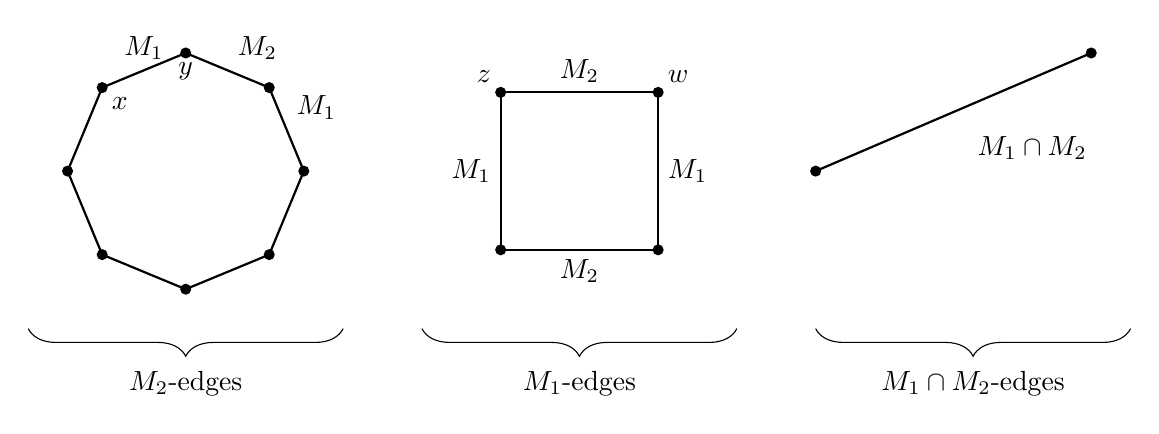
\begin{tikzpicture}
          % Left polygon (octagon)
          \foreach \i in {1,...,8} {
              \coordinate (p\i) at ({360/8 * \i}:1.5);
              \fill (p\i) circle (2pt);
          }
          \draw[thick] (p1) -- (p2) node[midway, above right] {$M_2$}
                      -- (p3) node[midway, above] {$M_1$}
                      -- (p4) -- (p5) -- (p6) -- (p7) -- (p8)
                      -- cycle node[midway, above right] {$M_1$};
          \node[below right] at (p3) {$x$};
          \node[below] at (p2) {$y$};
          
          % Middle square
          \draw[thick] (4,-1) rectangle (6,1);
          \node[above left] at (4,1) {$z$};
          \node[above right] at (6,1) {$w$};
          \node[below left] at (4,-1) {};
          \node[below right] at (6,-1) {};
          \draw (4,1) -- (6,1) node[midway, above] {$M_2$};
          \draw (6,1) -- (6,-1) node[midway, right] {$M_1$};
          \draw (6,-1) -- (4,-1) node[midway, below] {$M_2$};
          \draw (4,-1) -- (4,1) node[midway, left] {$M_1$};
          \fill (4,1) circle (2pt);
          \fill (6,1) circle (2pt);
          \fill (6,-1) circle (2pt);
          \fill (4,-1) circle (2pt);
          
          % Right diagonal line
          \draw[thick] (8,0) -- (11.5,1.5) node[midway, below right=5pt] {$M_1 \cap M_2$};
          \fill (8,0) circle (2pt);
          \fill (11.5,1.5) circle (2pt);
          
          \draw[decorate,decoration={brace,amplitude=10pt,mirror}] (-2,-2) -- (2,-2) node[midway,below=12pt] {$M_2$-edges};
          
          \draw[decorate,decoration={brace,amplitude=10pt,mirror}] (3,-2) -- (7,-2) node[midway,below=12pt] {$M_1$-edges};
          
          \draw[decorate,decoration={brace,amplitude=10pt,mirror}] (8,-2) -- (12,-2) node[midway,below=12pt] {$M_1 \cap M_2$-edges};
      
      
      \end{tikzpicture}
    \end{center}

        $M = M_1 \Delta M_2$ is a perfect matching in $G$:
        \begin{itemize}
          \item $M \subseteq E(G)$ $xy \notin M$, $zw \notin M$
          \item Every vertex is covered exactly once by $M$
        \end{itemize}
        \item If $xy$ and $zw$ belong to the same component, without loss of generality along the cycle
        the edges are ordered: $zw\dots xy \dots$ ($yx$ is a symmetric case)

        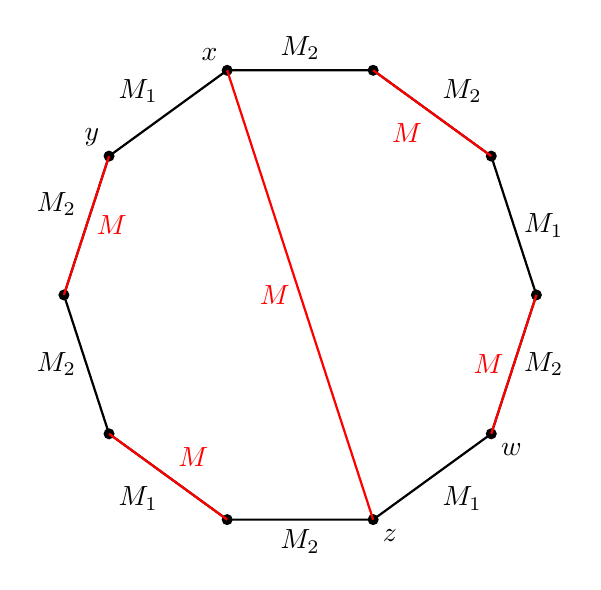
\begin{tikzpicture}

          % Define the coordinates for the octagon
          \foreach \i in {1,...,10} {
              \coordinate (p\i) at ({360/10 * (\i+2)}:3);
              \fill (p\i) circle (2pt);
          }
          
          % Draw the octagon with different labels on the edges
          \draw[thick] (p1) -- (p2) node[midway, above left] {$M_1$}
                      -- (p2) -- (p3) node[midway, above left] {$M_2$}
                      -- (p3) -- (p4) node[midway, left] {$M_2$}
                      -- (p4) -- (p5) node[midway, below left] {$M_1$}
                      -- (p5) -- (p6) node[midway, below] {$M_2$}
                      -- (p6) -- (p7) node[midway, below right] {$M_1$}
                      -- (p7) -- (p8) node[midway, right] {$M_2$}
                      -- (p8) -- (p9) node[midway, right] {$M_1$}
                      -- (p9) -- (p10) node[midway, above right] {$M_2$}
                      -- (p10) -- (p1) node[midway, above] {$M_2$};

          \draw[thick, red] (p1) -- (p6) node[midway, left] {$M$};
          \draw[thick, red] (p2) -- (p3) node[midway, right] {$M$};
          \draw[thick, red] (p4) -- (p5) node[midway, above right] {$M$};
          \draw[thick, red] (p7) -- (p8) node[midway, left] {$M$};
          \draw[thick, red] (p9) -- (p10) node[midway, below left] {$M$};
      
          % Label the vertices x, y, z, w
          \node[above left] at (p1) {$x$};
          \node[above left] at (p2) {$y$};
          \node[below right] at (p7) {$w$};
          \node[below right] at (p6) {$z$};
      
      \end{tikzpicture}
        
      \end{itemize}
    \end{enumerate}
  \end{itemize}
\end{proof}

\noindent\textbf{Borge-Tutte formula}:
A maximum matching in $G$ leaves exactly
\[\max_{S \subseteq V(G)}\{ o(G-S) - |S| \}\]
uncovered vertices. Equivalently:
\[ \alpha'(G) = \frac{1}{2}\left( n- \max_{S \subseteq V(G)}\{ o(G-S) - |S| \} \right)\]
\end{document}